\documentclass[sigconf,nonacm]{acmart}

%% Enable subfigures
\usepackage{subfigure}
%% Enable numbers in scientific format.
\usepackage{siunitx}
%% Enable enumerate start from.
\usepackage{enumitem}

%% Enable theorems
\newtheorem{theorem}{Theorem}[section]
\newtheorem{lemma}[theorem]{Lemma}

%% Enable algorithms
\usepackage{algorithm}
\usepackage[noend]{algpseudocode}
\let\ReturnInline\Return
\renewcommand{\Return}{\State\ReturnInline}
\algrenewcommand\algorithmicrequire{$\rhd$}
\algrenewcommand\algorithmicensure{$\square$}

%% Fonts used in the template cannot be substituted; margin 
%% adjustments are not allowed.
\AtBeginDocument{%
  \providecommand\BibTeX{{%
    \normalfont B\kern-0.5em{\scshape i\kern-0.25em b}\kern-0.8em\TeX}}}

%% Rights management information.
\setcopyright{acmcopyright}
\copyrightyear{2018}
\acmYear{2018}
\acmDOI{XXXXXXX.XXXXXXX}

%% These commands are for a PROCEEDINGS abstract or paper.
\acmConference[Conference acronym 'XX]{Make sure to enter the correct
  conference title from your rights confirmation emai}{June 03--05,
  2018}{Woodstock, NY}
%% Title of the proceedings is different from ``Proceedings of ...''?
% \acmBooktitle{Woodstock '18: ACM Symposium on Neural Gaze Detection,
%  June 03--05, 2018, Woodstock, NY} 
% \acmPrice{15.00}
% \acmISBN{978-1-4503-XXXX-X/18/06}

%% Submission ID.
% \acmSubmissionID{123-A56-BU3}

%% Use the "author year" style of citations and references?
% \citestyle{acmauthoryear}

%% Message
\newcommand{\kk}[1]{{{\color{red} #1}}}
\newcommand{\ds}[1]{{{\color{blue} #1}}}
\newcommand{\su}[1]{{{\color{green} #1}}}

%% Ignore block
\newcommand{\ignore}[1]{}

%% Macros
\newcommand{\Lou}{\textit{Louvain}}
\newcommand{\LPA}{\textit{LPA}}
\newcommand{\Hyb}{\textit{Hybrid Louvain-LPA}}
\newcommand{\Sta}{\textit{Static}}
\newcommand{\Nai}{P-ND}
\newcommand{\DelOrg}{\textit{$\Delta$-screening}}
\newcommand{\Del}{P-DDS}
\newcommand{\Fro}{P-DF}
\newcommand{\StaLou}{\textit{Static Louvain}}
\newcommand{\NaiLou}{$\text{P-ND}_\text{L}$}
\newcommand{\DelLou}{$\text{P-DDS}_\text{L}$}
\newcommand{\FroLou}{$\text{P-DF}_\text{L}$}
\newcommand{\StaLPA}{\textit{Static LPA}}
\newcommand{\NaiLPA}{$\text{P-ND}_\text{LPA}$}
\newcommand{\DelLPA}{$\text{P-DDS}_\text{LPA}$}
\newcommand{\FroLPA}{$\text{P-DF}_\text{LPA}$}
\newcommand{\FroHyb}{$\text{P-DF}_\text{H}$}




\begin{document}

%% Full title of the paper.
\title[GVE-LPA: Fast Label Propagation Algorithm (LPA) for Community Detection in Shared Memory Setting]{GVE-LPA: Fast Label Propagation Algorithm (LPA) for Community Detection in Shared Memory Setting}

%% Short title to be used in page headers (optional).
% \title[short title]{full title}
% \subtitle{Something other than the title}

%% Authors and their affiliations.
\author{Subhajit Sahu}
\email{subhajit.sahu@research.iiit.ac.in}
\affiliation{%
  \institution{IIIT Hyderabad}
  \streetaddress{Professor CR Rao Rd, Gachibowli}
  \city{Hyderabad}
  \state{Telangana}
  \country{India}
  \postcode{500032}
}

%% Concise author list in page headers.
%\renewcommand{\shortauthors}{Sahu, Kothapalli, and Banerjee, et al.}

%% Show page numbers.
\settopmatter{printfolios=true}

%% Short summary of the work to be presented in the article.
\begin{abstract}
Community detection is the problem of identifying natural divisions in networks. Efficient parallel algorithms for this purpose are crucial in various applications, particularly as datasets grow to substantial scales. This technical report presents an optimized parallel implementation of the Label Propagation Algorithm (LPA), a high speed community detection method, for shared memory multicore systems. On a server equipped with dual 16-core Intel Xeon Gold 6226R processors, our LPA, which we term as GVE-LPA, outperforms FLPA, igraph LPA, and NetworKit LPA by $97,000\times$, $118,000\times$, and $40\times$ respectively - achieving a processing rate of $1.4 B$ edges/s on a $3.8 B$ edge graph. In addition, GVE-LPA scales at a rate of $1.7\times$ every doubling of threads.
\end{abstract}

%% The code below is generated by the tool at http://dl.acm.org/ccs.cfm.
\begin{CCSXML}
<ccs2012>
<concept>
<concept_id>10003752.10003809.10010170</concept_id>
<concept_desc>Theory of computation~Parallel algorithms</concept_desc>
<concept_significance>500</concept_significance>
</concept>
<concept>
<concept_id>10003752.10003809.10003635</concept_id>
<concept_desc>Theory of computation~Graph algorithms analysis</concept_desc>
<concept_significance>500</concept_significance>
</concept>
</ccs2012>
\end{CCSXML}

% \ccsdesc[500]{Theory of computation~Parallel algorithms}
% \ccsdesc[500]{Theory of computation~Graph algorithms analysis}

%% Pick words that accurately describe the work being presented.
\keywords{Community detection, Parallel Label Propagation Algorithm (LPA)}

% \received{20 February 2007}
% \received[revised]{12 March 2009}
% \received[accepted]{5 June 2009}



%% Process the author and title information.
\maketitle

\section{Introduction}
\label{sec:introduction}
Community detection is the problem of identifying cohesive groups of vertices, also known as clusters, in complex networks that minimize cuts and maximize internal density \cite{garza2019community}. This NP-hard problem finds applications in various domains, including drug discovery, protein annotation, topic exploration, anomaly detection, and criminal identification. Communities identified are intrinsic when based on network topology alone, and are disjoint when each vertex belongs to only one community \cite{com-gregory10}.\ignore{One of the difficulties in the community detection problem is the lack of apriori knowledge on the number and size distribution of communities \cite{com-blondel08}.} The \textit{Label Propagation Algorithm (LPA)}, also known as RAK, \cite{com-blondel08} is a popular heuristic-based approach for community detection, with the modularity metric \cite{com-newman06} being used to measure the quality of communities identified.

In the past few years, there has been an unprecedented surge in the gathering of data and the depiction of their interconnections through graphs. This surge has underscored the need for devising efficient parallel algorithms tailored for identifying communities within massive networks. The significance of the multicore/shared memory environment in this context is paramount, owing to its energy-efficient nature and the prevalence of hardware equipped with substantial DRAM capacities.\ignore{Optimizing parallel community detection algorithms for modern hardware architectures can yield notable performance benefits and competitive advantages across applications. However, many of the current algorithms for community detection are challenging to parallelize due to their irregular and inherently sequential nature \cite{com-halappanavar17}, in addition to the complexities of handling concurrency, optimizing data access, reducing contention, minimizing load imbalance.} Existing studies on LPA propose algorithmic optimizations and parallelization techniques, but do not study efficient data structures for picking the most weighted label, to the best of our knowledge. Moreover, the proposed techniques are scattered over a number of papers\ignore{, making it difficult for a reader to get a grip over them}.




\subsection{Our Contributions}

This report introduces GVE-LPA\footnote{https://github.com/puzzlef/rak-communities-openmp}, an optimized parallel implementation of LPA for shared memory multicores. On a machine with two 16-core Intel Xeon Gold 6226R processors, GVE-LPA outperforms FLPA, igraph LPA, and NetworKit LPA by $97,000\times$, $118,000\times$, and $40\times$ respectively. GVE-LPA is on average $5.4\times$ faster than GVE-Louvain, and achieves a processing rate of $1.4 B$ edges/s on a $3.8 B$ edge graph. With doubling of threads, GVE-LPA exhibits an average performance scaling of $1.7\times$.




%% - Use --- for a dash.
%% - Use ``camera-ready'' for quotes.
%% - Use {\itshape very} or \textit{very} for italicized text.
%% - Use \verb|acmart| or {\verb|acmart|} for mono-spaced text.
%% - Use \url{https://capitalizemytitle.com/} for URLs.
%% - Use {\bfseries Do not modify this document.} for important boldface details.
%% - Use \ref{fig:name} for referencing.

%% For a block of pre-formatted text: 
% \begin{verbatim}
%   \renewcommand{\shortauthors}{McCartney, et al.}
% \end{verbatim}

%% For a list of items:
% \begin{itemize}
% \item the ``ACM Reference Format'' text on the first page.
% \item the ``rights management'' text on the first page.
% \item the conference information in the page header(s).
% \end{itemize}

%% For a table:
% \begin{table}
%   \caption{Frequency of Special Characters}
%   \label{tab:freq}
%   \begin{tabular}{ccl}
%     \toprule
%     Non-English or Math&Frequency&Comments\\
%     \midrule
%     \O & 1 in 1,000& For Swedish names\\
%     $\pi$ & 1 in 5& Common in math\\
%     \$ & 4 in 5 & Used in business\\
%     $\Psi^2_1$ & 1 in 40,000& Unexplained usage\\
%   \bottomrule
% \end{tabular}
% \end{table}

%% For a full-width table:
% \begin{table*}
%   \caption{Some Typical Commands}
%   \label{tab:commands}
%   \begin{tabular}{ccl}
%     \toprule
%     Command &A Number & Comments\\
%     \midrule
%     \texttt{{\char'134}author} & 100& Author \\
%     \texttt{{\char'134}table}& 300 & For tables\\
%     \texttt{{\char'134}table*}& 400& For wider tables\\
%     \bottomrule
%   \end{tabular}
% \end{table*}


%% For inline math:
% \begin{math}
%   \lim_{n\rightarrow \infty}x=0
% \end{math},

%% For a numbered equation:
% \begin{equation}
%   \lim_{n\rightarrow \infty}x=0
% \end{equation}

%% For an unnumbered equation:
% \begin{displaymath}
%   \sum_{i=0}^{\infty} x + 1
% \end{displaymath}

%% For a figure:
% \begin{figure}[h]
%   \centering
%   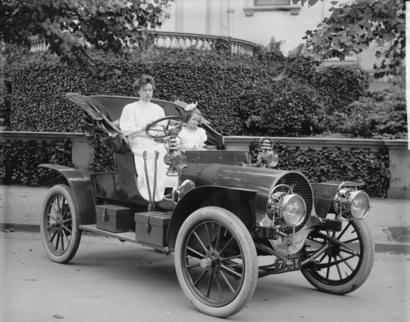
\includegraphics[width=\linewidth]{inc/sample-franklin}
%   \caption{1907 Franklin Model D roadster. Photograph by Harris \&
%     Ewing, Inc. [Public domain], via Wikimedia
%     Commons. (\url{https://goo.gl/VLCRBB}).}
%   \Description{A woman and a girl in white dresses sit in an open car.}
% \end{figure}

%% For a teaser figure.
% \begin{teaserfigure}
%   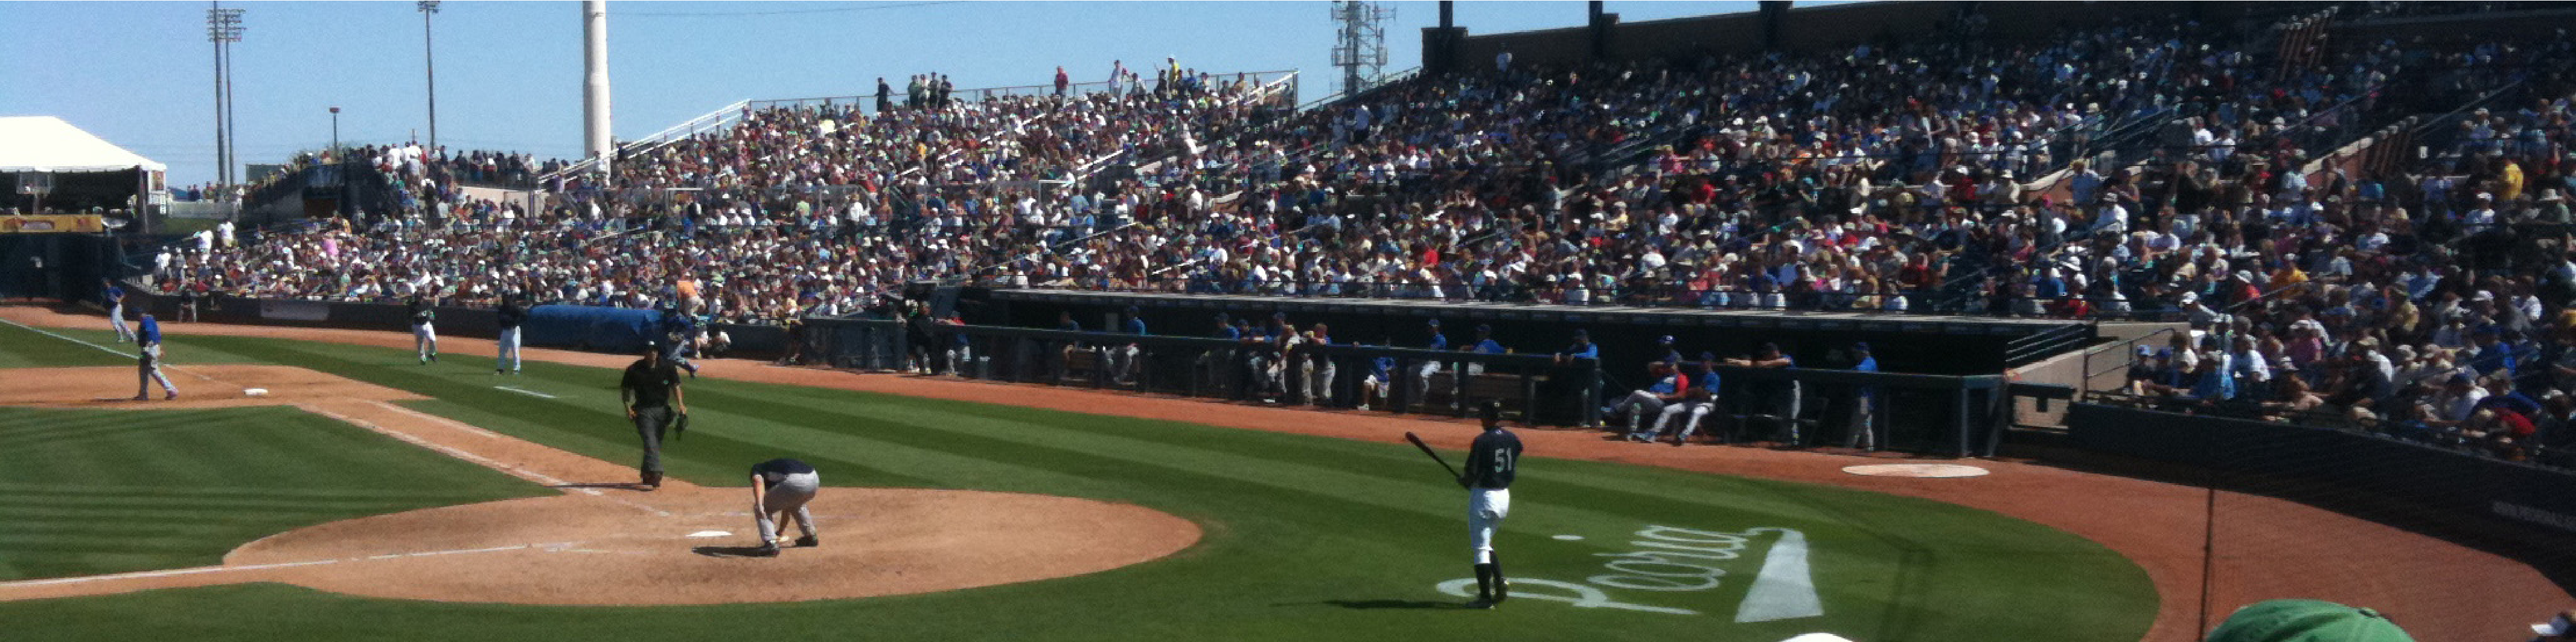
\includegraphics[width=\textwidth]{sampleteaser}
%   \caption{figure caption}
%   \Description{figure description}
% \end{teaserfigure}


\section{Related work}
\label{sec:related}
The \textit{Label Propagation Algorithm (LPA)} is a greedy modularity-optimization based community detection algorithm, and is introduced by Blondel et al. from the University of LPA \cite{com-blondel08}. It identifies communities with resulting high modularity, and is thus widely favored \cite{com-lancichinetti09}. Algorithmic improvements proposed for the original algorithm include early pruning of non-promising candidates (leaf vertices) \cite{com-ryu16, com-halappanavar17, com-zhang21, com-you22}, attempting local move only on likely vertices \cite{com-ryu16, com-ozaki16, com-zhang21, com-shi21}, ordering of vertices based on node importance \cite{com-aldabobi22}, moving nodes to a random neighbor community \cite{com-traag15}, threshold scaling \cite{com-lu15, com-naim17, com-halappanavar17}, threshold cycling \cite{com-ghosh18}, subnetwork refinement \cite{com-waltman13, com-traag19}, multilevel refinement \cite{com-rotta11, com-gach14, com-shi21}, and early termination \cite{com-ghosh18}.

To parallelize the LPA algorithm, a number of strategies have been attempted. These include using heuristics to break the sequential barrier \cite{com-lu15}, ordering vertices via graph coloring \cite{com-halappanavar17}, performing iterations asynchronously \cite{com-que15, com-shi21}, using adaptive parallel thread assignment \cite{com-fazlali17, com-naim17, com-sattar19, com-mohammadi20}, parallelizing the costly first iteration \cite{com-wickramaarachchi14}, using vector based hashtables \cite{com-halappanavar17}, and using sort-reduce instead of hashing \cite{com-cheong13}\ignore{, using simple partitions based of vertex ids \cite{com-cheong13, com-ghosh18}, and identifying and moving ghost/doubtful vertices \cite{com-zeng15, com-que15, com-bhowmik19, com-bhowmick22}}. Platforms used range from an AMD multicore system \cite{com-fazlali17}, and Intel’s Knight's Landing, Haswell \cite{com-gheibi20}, SkylakeX, and Cascade Lake \cite{part-hossain21}. Other approaches include the use of MapReduce in a BigData batch processing framework \cite{com-zeitz17}. It should however be noted though that community detection methods such as the LPA that rely on modularity maximization are known to suffer from resolution limit problem. This prevents identification of communities of certain sizes \cite{com-ghosh19}.

A few open source implementations and software packages have been developed for community detection. Vite \cite{ghosh2018scalable} is a distributed memory parallel implementation of the LPA method that incorporates several heuristics to enhance performance while maintaining solution quality, while Grappolo \cite{com-halappanavar17} is a shared memory parallel implementation. NetworKit \cite{staudt2016networkit} is a software package designed for analyzing the structural aspects of graph data sets with billions of connections. It is implemented as a hybrid with C++ kernels and a Python frontend, and includes a parallel implementation of the LPA algorithm.


\section{Preliminaries}
\label{sec:preliminaries}
Consider an undirected graph $G(V, E, w)$, where $V$ is the set of vertices, $E$ is the set of edges, and $w_{ij} = w_{ji}$ represents the weight associated with each edge. For unweighted graphs, we assume a unit weight for each edge, i.e., $w_{ij} = 1$. The neighbors of a vertex $i$ are denoted as $J_i = {j\ |\ (i, j) \in E}$, the weighted degree of each vertex as $K_i = \sum_{j \in J_i} w_{ij}$, the total number of vertices as $N = |V|$, the total number of edges as $M = |E|$, and the sum of edge weights in the undirected graph as $m = \sum_{i, j \in V} w_{ij}/2$.




\subsection{Community detection}

Disjoint community detection involves the identification of a community membership mapping, $C: V \rightarrow \Gamma$, where each vertex $i \in V$ is assigned a community ID $c \in \Gamma$, with $\Gamma$ representing the set of community IDs. We denote the vertices belonging to a community $c \in \Gamma$ as $V_c$, and the community to which a vertex $i$ belongs as $C_i$. Additionally, we denote the neighbors of vertex $i$ within community $c$ as $J_{i \rightarrow c} = {j\ |\ j \in J_i\ and\ C_j = c}$, the sum of edge weights for those neighbors as $K_{i \rightarrow c} = \sum_{j \in J_{i \rightarrow c}} w_{ij}$, the edge weight within a community $c$ as $\sigma_c = \sum_{(i, j) \in E\ and\ C_i = C_j = c} w_{ij}$, and the total edge weight of a community $c$ as $\Sigma_c = \sum_{(i, j) \in E\ and\ C_i = c} w_{ij}$ \cite{com-leskovec21}.




\subsection{Modularity}

Modularity functions as a metric for evaluating the quality of communities identified by heuristic-based community detection algorithms. It is calculated as the difference between the fraction of edges within communities and the expected fraction under random edge distribution. It lies in a range of $[-0.5, 1]$, where higher values signify superior quality \cite{com-brandes07}.\ignore{The optimization of this metric theoretically leads to the optimal grouping \cite{com-newman04, com-traag11}.} The modularity $Q$ for the identified communities is computed using Equation \ref{eq:modularity}, where $\delta$ denotes the Kronecker delta function ($\delta (x,y)=1$ if $x=y$, $0$ otherwise).\ignore{The \textit{delta modularity} of moving a vertex $i$ from community $d$ to community $c$, denoted as $\Delta Q_{i: d \rightarrow c}$, can be computed using Equation \ref{eq:delta-modularity}.}

\begin{equation}
\label{eq:modularity}
  Q
  = \frac{1}{2m} \sum_{(i, j) \in E} \left[w_{ij} - \frac{K_i K_j}{2m}\right] \delta(C_i, C_j)
  = \sum_{c \in \Gamma} \left[\frac{\sigma_c}{2m} - \left(\frac{\Sigma_c}{2m}\right)^2\right]
\end{equation}

\ignore{\begin{equation}
\label{eq:delta-modularity}
  \Delta Q_{i: d \rightarrow c}
  = \frac{1}{m} (K_{i \rightarrow c} - K_{i \rightarrow d}) - \frac{K_i}{2m^2} (K_i + \Sigma_c - \Sigma_d)
\end{equation}}




\subsection{Label Progagation Algorithm (LPA)}
\label{sec:about-rak}

LPA \cite{com-raghavan07} is a popular diffusion-based method for identifying communities of medium quality in large networks. It is simpler, faster, and more scalable compared to the Louvain method \cite{com-blondel08}. In LPA, each vertex $i$ is starts with a unique label (community id) $C_i$. During each iteration, vertices adopt the label with the highest interconnecting weight, as shown in Equation \ref{eq:lpa}. Through this iterative process, a consensus among densely connected groups of vertices is achieved, forming communities. The algorithm converges when at least $1-\tau$ fraction of vertices (where $\tau$ is the tolerance parameter) maintain their community membership. LPA exhibits a time complexity of $O(L |E|)$ and a space complexity of $O(|V| + |E|)$, with $L$ denoting the number of iterations performed \cite{com-raghavan07}. We have experimented with COPRA \cite{com-gregory10}, SLPA \cite{com-xie11}, and LabelRank \cite{com-xie13}, but found LPA to be the most performant, while yielding communities of equivalent quality \cite{sahu2023selecting}.

\begin{equation}
\label{eq:lpa}
  C_i =\ \underset{c\ \in \ \Gamma}{\arg\max} { \sum_{j \in J_i\ |\ C_j = c} w_{ij} }
\end{equation}


\section{Approach}
\label{sec:approach}
\subsection{Optimizations for LPA}
\label{sec:lpa}

We use a parallel implementation of LPA and experiment with different optimizations and parameter settings. We use the \textit{asynchronous} version of LPA, wherein threads operate independently on distinct regions of the graph. This facilitates quicker convergence, but may introduce greater variability in the final result. Further, we observe that parallel LPA obtains communities of higher quality than its sequential implementation, possibly due to randomization. We allocate a separate hashtable per thread to keep track of the total weight of each unique label linked to a vertex.

Our optimizations include using OpenMP's \verb|dynamic| loop schedule, setting an initial tolerance of $0.05$, enabling vertex pruning, employing the strict version of LPA, and using fast collision-free per-thread hashtables which are well separated in their memory addresses (\textit{Far-KV}). See below for the details on each optimization.

We evaluate multiple alternatives for each optimization, and show the relative time and the relative modularity of communities obtained by each alternative in Figure \ref{fig:rak-opt}. We perform these tests on every graph in the dataset (refer to Table \ref{tab:dataset}), conducting them five times on each graph to minimize the influence of noise. We then calculate the geometric mean for the runtime and arithmetic mean for the modularity, and represent them as ratios within each optimization category.


\subsubsection{Adjusting OpenMP loop schedule}

We attempt \textit{static}, \textit{dynamic}, \textit{guided}, and \textit{auto} loop scheduling approaches of OpenMP (each with a chunk size of $2048$) to parallelize LPA. We consider OpenMP's \verb|dynamic| loop schedule to be the best choice, due to its ability of work balancing among threads, and because it yields a runtime reduction of $27\%$ when compared to OpenMP's \textit{auto} loop schedule, while incurring only a $0.7\%$ reduction in the modularity of obtained communities (likely to be just noise).


\subsubsection{Limiting the number of iterations}

Restricting the number of iterations of LPA can ensure its termination within a reasonable number of iterations, but choosing a small limit may worsen the quality of communities obtained. Our results suggest that limiting the maximum number of iterations to $20$ strikes a good balance between runtime and modularity.


\subsubsection{Adjusting tolerance}

Using a small tolerance allows the algorithm to explore broader possibilities for community assignments, but comes at the cost of increased runtime. We find an initial tolerance of $0.05$ to be suitable. A tolerance of $0.1$ may also be acceptable, but provides a very small gain in performance when compared to a tolerance of $0.05$.


\subsubsection{Vertex pruning}

Vertex pruning is a method utilized to minimize unnecessary computation. In this approach, when a vertex alters its community, it assigns its neighbors for processing. Once a vertex has been processed, it is labeled as ineligible for further processing. However, this procedure incurs an additional overhead due to the marking and unmarking of vertices. Based on our findings, the employment of vertex pruning justifies this overhead and results in a performance enhancement of $17\%$. An illustration of vertex pruning optimization is shown in Figure \ref{fig:rak-pruning}.

\begin{figure}[hbtp]
  \centering
  \subfigure{
    \label{fig:rak-pruning--all}
    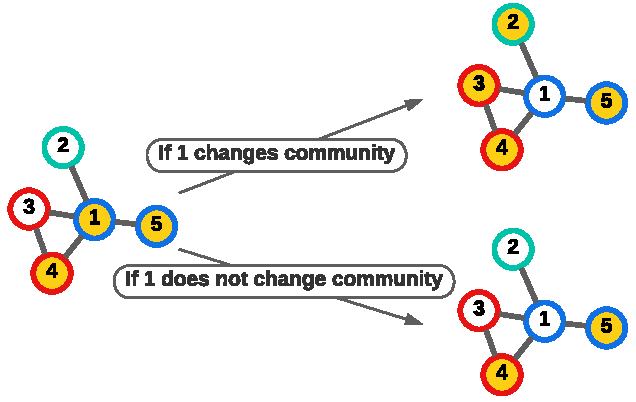
\includegraphics[width=0.78\linewidth]{out/rak-pruning.pdf}
  } \\[-2ex]
  \caption{Illustration of vertex pruning optimization: After processing vertex $1$, it's unmarked. If vertex $1$ changes its community, its neighbors are marked for processing. Community membership of each vertex is depicted by border color, and marked vertices are highlighted in yellow \cite{sahu2023gvelouvain}.}
  \label{fig:rak-pruning}
\end{figure}



\subsubsection{Picking the best label}

When there exist multiple labels connected to a vertex with maximum weight, we may randomly pick one of them (non-strict LPA), or pick only the first of them (strict LPA). We implement non-strict LPA using a simple modulo operator on the label id, as we observe that using \textit{xorshift} based random number generator does not provide any advantage. Results indicate that the strict version of LPA is $1.5\times$ faster than the non-strict approach, while also offering a gain in modularity of $2.1\%$.


\subsubsection{Hashtable design}

One can utilize C++'s inbuilt map as per-thread (independent) hashtables for the LPA algorithm. However, this exhibits poor performance. Therefore, we employ a key-list and a collision-free full-size values array to dramatically improve performance. However, if the memory addresses of the hashtables are nearby (\textit{Close-KV}), even if each thread uses its own hashtable exclusively, the performance is not as high. This is possibly due to false cache-sharing. Alternatively, if we ensure that the memory address of each hashtable is farther away (\textit{Far-KV}), the performance improves. Our results indicate that \textit{Far-KV} has the best performance and is $15.8\times$ times faster than \textit{Map}, and $2.6\times$ times faster than \textit{Close-KV} with LPA. An illustration of \textit{Far-KV} hashtable is in Figure \ref{fig:rak-hashtable}.

\begin{figure}[hbtp]
  \centering
  \subfigure{
    \label{fig:rak-hashtable--all}
    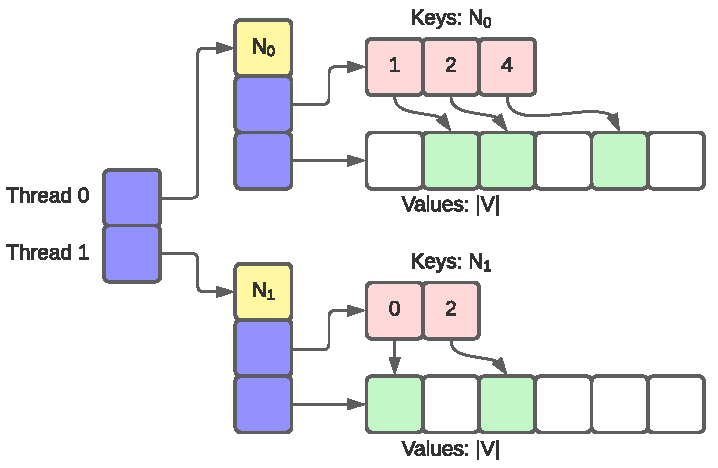
\includegraphics[width=0.88\linewidth]{out/rak-hashtable.pdf}
  } \\[-2ex]
  \caption{Illustration of collision-free per-thread hashtables that are well separated in their memory addresses (Far-KV), for two threads. Each hashtable consists of a keys vector, values vector (of size $|V|$), and a key count ($N_0$/$N_1$). The value associated with each key is stored/accumulated in the index pointed by the key. As the key count of each hashtable is updated independently, we allocate it separately on the heap to avoid false cache sharing \cite{sahu2023gvelouvain}.}
  \label{fig:rak-hashtable}
\end{figure}

\begin{figure*}[hbtp]
  \centering
  \subfigure{
    \label{fig:rak-opt--all}
    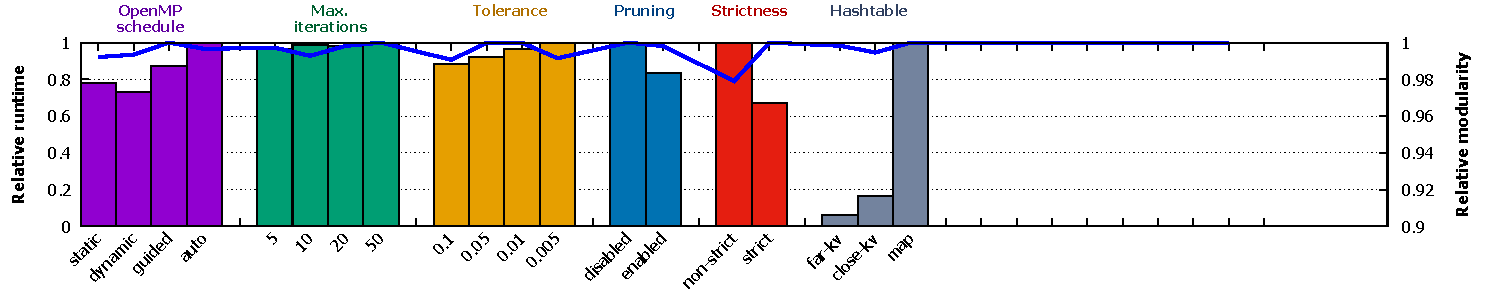
\includegraphics[width=0.98\linewidth]{out/rak-opt.pdf}
  } \\[-2ex]
  \caption{Impact of\ignore{various} parameter controls and optimizations on the runtime and result quality (modularity) of LPA. We show the impact of each optimization upon the relative runtime on the left Y-axis, and upon the relative modularity on the right Y-axis.}
  \label{fig:rak-opt}
\end{figure*}





\subsection{Our optimized LPA implementation}

We now explain the implementation of GVE-LPA in Algorithm \ref{alg:rak}. Its main step is the \texttt{lpa()} function (lines \ref{alg:rak--main-begin}-\ref{alg:rak--main-begin}), which takes the input graph $G$ and assigns community memberships (or labels) $C$ to each vertex. In lines \ref{alg:rak--init-begin}-\ref{alg:rak--init-end}, we first initialize the labels $C$ of each vertex in $G$, and mark all vertices as unprocessed. We then perform iterations to propagate labels based on the weighted influence of neighboring vertices, limited to $MAX\_ITERATIONS$ (lines \ref{alg:rak--iters-begin}-\ref{alg:rak--iters-end}). In each iteration, we invoke the \texttt{lpaMove()} function to perform label propagation, and count the number of nodes with updated labels $\Delta N$ (line \ref{alg:rak--propagate}). If the ratio of $\Delta N$ to the total number of nodes $N$ is within a specified tolerance $\tau$, convergence has been achieved, and we terminate the loop (line \ref{alg:rak--converged}). Upon completing all iterations, we return the final labels $C$ (line \ref{alg:rak--main-return}).

\begin{algorithm}[hbtp]
\caption{GVE-LPA: Our parallel Label Propagation Algorithm (LPA).}
\label{alg:rak}
\begin{algorithmic}[1]
\Require{$G'$: Input graph}
\Require{$C$: Community membership of each vertex}
\Require{$G'$: Input/super-vertex graph}
\Require{$C'$: Community membership of each vertex in $G'$}
\Require{$K'$: Total edge weight of each vertex}
\Require{$\Sigma'$: Total edge weight of each community}
\Ensure{$G'_{C'}$: Community vertices (CSR)}
\Ensure{$H_t$: Collision-free per-thread hashtable}
\Ensure{$l_i$: Number of iterations performed (per pass)}
\Ensure{$l_p$: Number of passes performed}
\Ensure{$\tau$: Per iteration tolerance}
\Ensure{$\tau_{agg}$: Aggregation tolerance}

\Statex

\Function{louvain}{$G$} \label{alg:louvain--begin}
  \State Vertex membership: $C \gets [0 .. |V|)$ \textbf{;} $G' \gets G$ \label{alg:louvain--initialization}
  \ForAll{$l_p \in [0 .. \text{\small{MAX\_PASSES}})$} \label{alg:louvain--passes-begin}
    \State $\Sigma' \gets K' \gets vertexWeights(G')$ \textbf{;} $C' \gets [0 .. |V'|)$ \label{alg:louvain--reset-weights}
    \State Mark all vertices in $G'$ as unprocessed \label{alg:louvain--reset-affected}
    \State $l_i \gets louvainMove(G', C', K', \Sigma')$ \label{alg:louvain--local-move}
    \If{$l_i \le 1$} \textbf{break} \Comment{Globally converged?} \label{alg:louvain--globally-converged}
    \EndIf
    \State $|\Gamma|, |\Gamma_{old}| \gets$ Number of communities in $C$, $C'$
    \If{$|\Gamma|/|\Gamma_{old}| > \tau_{agg}$} \textbf{break} \Comment{Low shrink?} \label{alg:louvain--aggregation-tolerance}
    \EndIf
    \State $C' \gets$ Renumber communities in $C'$ \label{alg:louvain--renumber}
    \State $C \gets$ Lookup dendrogram using $C$ to $C'$ \label{alg:louvain--lookup}
    \State $G' \gets louvainAggregate(G', C')$ \label{alg:louvain--aggregate}
    \State $\tau \gets \tau / \text{\small{TOLERANCE\_DROP}}$ \Comment{Threshold scaling} \label{alg:louvain--threshold-scaling}
  \EndFor \label{alg:louvain--passes-end}
  \State $C \gets$ Lookup dendrogram using $C$ to $C'$ \label{alg:louvain--lookup-last}
  \Return{$C$} \label{alg:louvain--return}
\EndFunction \label{alg:louvain--end}
\end{algorithmic}
\end{algorithm}


The \texttt{lpaMove()} function (lines \ref{alg:rak--move-begin}-\ref{alg:rak--move-end}) iterates over unprocessed vertices in parallel. For each unprocessed vertex $i$ in the graph $G$, we mark $i$ as processed - vertex pruning (line \ref{alg:rak--prune}), obtain the total edge weight of connected labels in per-thread hashtable $H_t$ with the \texttt{scanCommunities()} function \ref{alg:rak--scan}, and select the most weighted label $c^*$ (line \ref{alg:rak--best-community}). If $c^*$ is not the same as the current label of $i$, we update the label of $i$, increment the count of changed vertices $\Delta N$, and mark the neighbors of $i$ as unprocessed for the next iteration (lines \ref{alg:rak--perform-move}-\ref{alg:rak--remark}). After having processed all vertices, we return the total number of vertices with updated labels $\Delta N$ (line \ref{alg:rak--move-return}). The \texttt{scanCommunities()} (lines \ref{alg:rak--scan-begin}-\ref{alg:rak--scan-end}) iterates over the neighbors of the current vertex $i$, excluding itself, and calculates the total weight of each label in the hashtable $H_t$.


\section{Evaluation}
\label{sec:evaluation}
\subsection{Experimental Setup}
\label{sec:setup}

We use a server that has two $16$-core x86-based Intel Xeon Gold 6226R processors running at $2.90$ GHz. Each core has an L1 cache of $1$ MB, an L2 cache of $16$ MB, and a shared L3 cache of $22$ MB. The machine has $93.4$ GB of system memory and runs on CentOS Stream 8. We use GCC 8.5 and OpenMP 4.5. Table \ref{tab:dataset} shows the graphs we use in our experiments. All of them are obtained from the SuiteSparse Matrix Collection \cite{suite19}.

\begin{table}[hbtp]
  \centering
  \caption{List of $13$ graphs obtained SuiteSparse Matrix Collection \cite{suite19} (directed graphs are marked with $*$). Here, $|V|$ is the number of vertices, $|E|$ is the number of edges (after adding reverse edges), $D_{avg}$ is the average degree, and $|\Gamma|$ is the number of communities obtained using LPA.\ignore{In the table, B refers to a billion, M refers to a million and K refers a thousand.}}
  \label{tab:dataset}
  \begin{tabular}{|c||c|c|c|c|}
    \toprule
    \textbf{Graph} &
    \textbf{\textbf{$|V|$}} &
    \textbf{\textbf{$|E|$}} &
    \textbf{\textbf{$D_{avg}$}} &
    \textbf{\textbf{$|\Gamma|$}} \\
    % \textbf{$1 - \Gamma_G$} \\
    \midrule
    \multicolumn{5}{|c|}{\textbf{Web Graphs (LAW)}} \\ \hline
    indochina-2004$^*$ & 7.41M & 341M & 41.0 & 4.24K \\ \hline  % & \num{4.7e-4} & 2.9 GB
    uk-2002$^*$ & 18.5M & 567M & 16.1 & 42.8K \\ \hline  % & \num{9.6e-5} & 16 GB
    arabic-2005$^*$ & 22.7M & 1.21B & 28.2 & 3.66K \\ \hline  % & \num{5.5e-4} & 11 GB
    uk-2005$^*$ & 39.5M & 1.73B & 23.7 & 20.8K \\ \hline  % & \num{9.6e-5} & 16 GB
    webbase-2001$^*$ & 118M & 1.89B & 8.6 & 2.76M \\ \hline  % & \num{7.3e-7} & 18 GB
    it-2004$^*$ & 41.3M & 2.19B & 27.9 & 5.28K \\ \hline  % & \num{3.8e-4} & 19 GB
    sk-2005$^*$ & 50.6M & 3.80B & 38.5 & 3.47K \\ \hline  % & \num{5.8e-4} & 33 GB
    \multicolumn{5}{|c|}{\textbf{Social Networks (SNAP)}} \\ \hline
    com-LiveJournal & 4.00M & 69.4M & 17.4 & 2.54K \\ \hline  % & \num{7.9e-4} & 480 MB
    com-Orkut & 3.07M & 234M & 76.2 & 29 \\ \hline  % & \num{6.7e-2} & 1.7 GB
    \multicolumn{5}{|c|}{\textbf{Road Networks (DIMACS10)}} \\ \hline
    asia\_osm & 12.0M & 25.4M & 2.1 & 2.38K \\ \hline  % & \num{8.4e-4} & 200 MB
    europe\_osm & 50.9M & 108M & 2.1 & 3.05K \\ \hline  % & \num{6.6e-4} & 910 MB
    \multicolumn{5}{|c|}{\textbf{Protein k-mer Graphs (GenBank)}} \\ \hline
    kmer\_A2a & 171M & 361M & 2.1 & 21.2K \\ \hline  % & \num{9.4e-5} & 3.2 GB
    kmer\_V1r & 214M & 465M & 2.2 & 6.17K \\ \hline  % & \num{3.2e-4} & 4.2 GB
  \bottomrule
  \end{tabular}
\end{table}
% We convert directed graphs (marked with $*$) to undirected by duplicating edges in the reverse direction, and set the weight of each edge to $1$. and $F_{size}$ is size of the \textit{MatrixMarket} file

\begin{figure*}[hbtp]
  \centering
  \subfigure[Runtime in seconds (logarithmic scale) with \textit{FLPA}, \textit{igraph LPA}, \textit{NetworKit LPA}, and \textit{GVE-LPA}]{
    \label{fig:rak-compare--runtime}
    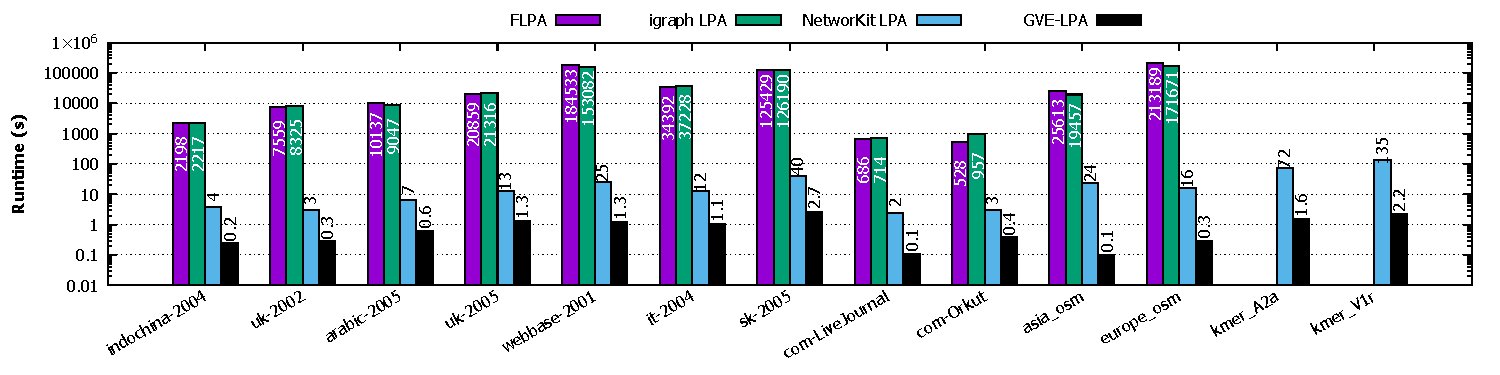
\includegraphics[width=0.98\linewidth]{out/rak-runtime.pdf}
  } \\[-0ex]
  \subfigure[Speedup (logarithmic scale) of \textit{GVE-LPA} with respect to \textit{FLPA}, \textit{igraph LPA}, \textit{NetworKit LPA}.]{
    \label{fig:rak-compare--speedup}
    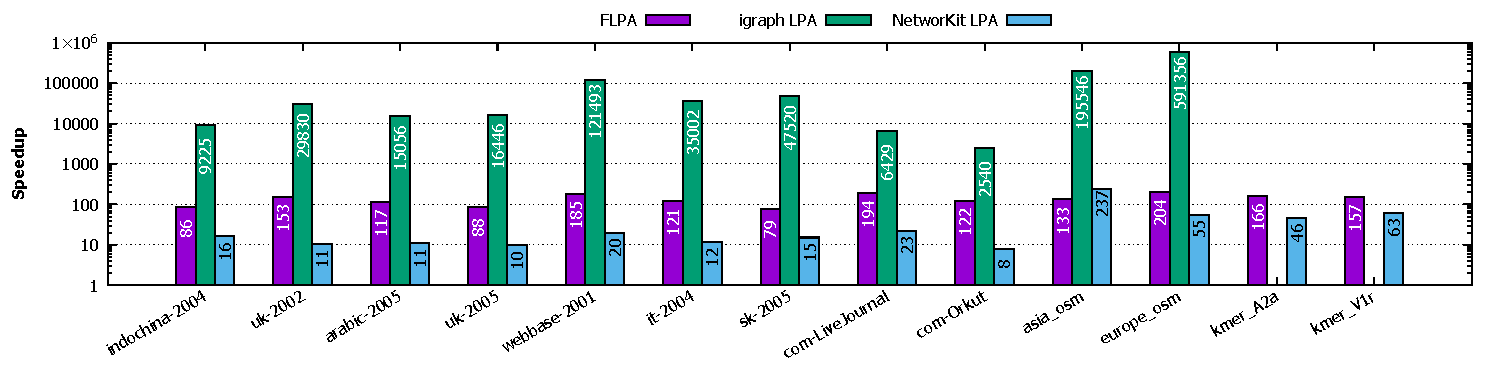
\includegraphics[width=0.98\linewidth]{out/rak-speedup.pdf}
  } \\[-0ex]
  \subfigure[Modularity of communities obtained with \textit{FLPA}, \textit{igraph LPA}, \textit{NetworKit LPA}, and \textit{GVE-LPA}.]{
    \label{fig:rak-compare--modularity}
    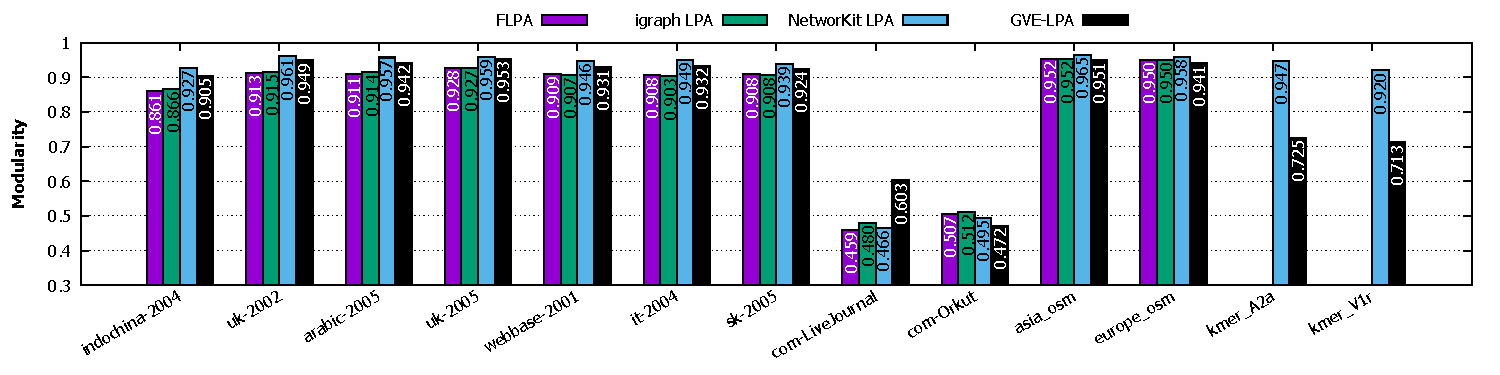
\includegraphics[width=0.98\linewidth]{out/rak-modularity.pdf}
  } \\[-2ex]
  \caption{Runtime\ignore{in seconds (logarithmic scale)}, speedup, and modularity of communities obtained with \textit{FLPA}, \textit{igraph LPA}, \textit{NetworKit LPA}, and \textit{GVE-LPA} for each graph\ignore{in the dataset}. \textit{FLPA} and \textit{igraph LPA} fail to run on \textit{kmer\_A2a} and \textit{kmer\_V1r} graphs, and thus their results are not shown.}
  \label{fig:rak-compare}
\end{figure*}





\subsection{Comparing Performance of GVE-LPA}

We now compare the performance of GVE-LPA with igraph LPA, FLPA, and NetworKit LPA. For Vite, we convert the graph datasets to Vite's binary graph format, run it on a single node\ignore{(Vite supports distributed community detection)} with threshold cycling/scaling optimization, and measure the reported average total time. For Grappolo, we measure the run it on the same system, and measure the reported total time. For NetworKit, we use a Python script to invoke \texttt{PLM} (Parallel Louvain Method), and measure the total time reported with \texttt{getTiming()}. For each graph, we measure the runtime of each implementation five times, for averaging. We also record the modularity of communities obtained, as reported by each implementation.

Figure \ref{fig:rak-compare--runtime} shows the runtimes of Vite (Louvain), Grappolo (Louvain), NetworKit Louvain, and GVE-Louvain on each graph in the dataset. Figure \ref{fig:rak-compare--speedup} shows the speedup of GVE-Louvain with respect to each implementation mentioned above. GVE-Louvain is on average $50\times$, $22\times$, and $20\times$ faster than Vite, Grappolo, and NetworKit respectively. On the \textit{sk-2005} graph, GVE-Louvain finds communities in $6.8$ seconds, and thus achieve a processing rate of $560$ million edges/s. Figure \ref{fig:rak-compare--modularity} shows the modularity of communities obtained with each implementation. GVE-Louvain on average obtains $3.1\%$ higher modularity than Vite (especially on web graphs), and $0.6\%$ lower modularity than Grappolo and NetworKit (especially on social networks with poor clustering).

\begin{figure}[hbtp]
  \centering
  \subfigure{
    \label{fig:rak-hardness--all}
    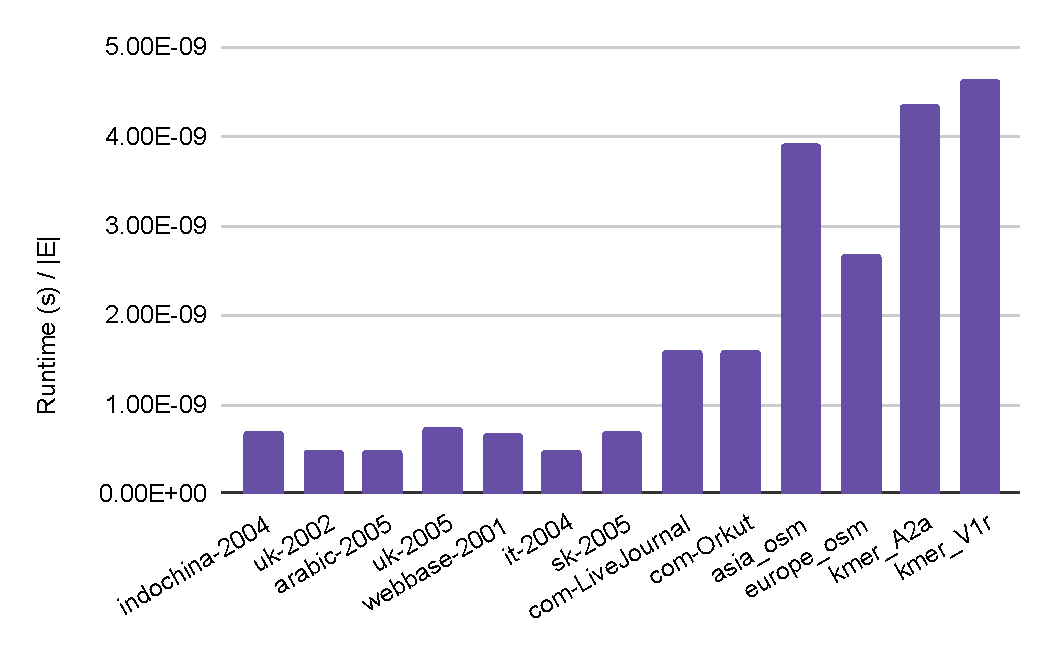
\includegraphics[width=0.98\linewidth]{out/rak-hardness.pdf}
  } \\[-2ex]
  \caption{Runtime $/ |E|$ factor with \textit{GVE-LPA} for each graph in the dataset.}
  \label{fig:rak-hardness}
\end{figure}

\begin{figure}[hbtp]
  \centering
  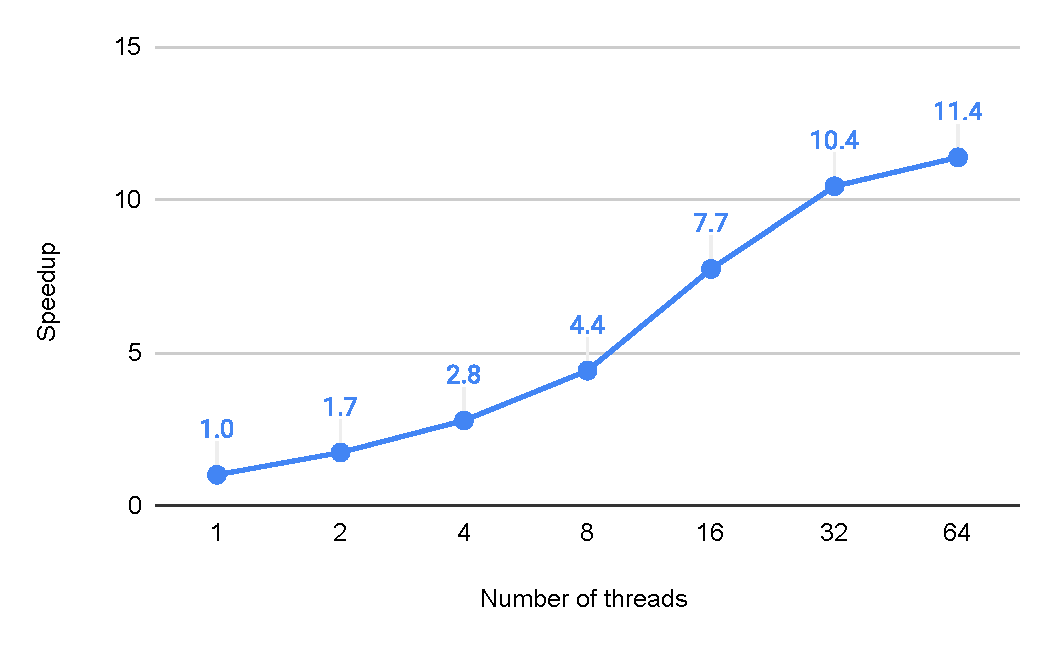
\includegraphics[width=0.98\linewidth]{out/rak-ss.pdf} \\[0ex]
  \caption{Average speedup of \textit{GVE-LPA} with increasing number of threads (in multiples of 2).}
  \label{fig:rak-ss}
\end{figure}





\subsection{Analyzing Performance of GVE-LPA}

The phase-wise and pass-wise split of GVE-Louvain is shown in Figures \ref{fig:louvain-splits--phase} and \ref{fig:louvain-splits--pass} respectively. Figure \ref{fig:louvain-splits--phase} indicates that GVE-Louvain spends most of the runtime in the local-moving phase on \textit{web graphs}, \textit{road networks}, and \textit{protein k-mer graphs}, while it devotes majority of the runtime in the aggregation phase on \textit{social networks}. The pass-wise split (Figure \ref{fig:louvain-splits--pass}) indicates that the first pass dominates runtime on high-degree graphs (\textit{web graphs} and \textit{social networks}), while subsequent passes prevail in execution time on low-degree graphs (\textit{road networks} and \textit{protein k-mer graphs}).

On average, $49\%$ of GVE-Louvain's runtime is spent in the local-moving phase, $35\%$ is spent in the aggregation phase, and $16\%$ is spent in other steps (initialization, renumbering communities, looking up dendrogram, and resetting communities) of the algorithm. Further, $67\%$ of the runtime is spent in the first pass of the algorithm, which is the most expensive pass due to the size of the original graph (later passes work on super-vertex graphs) \cite{com-wickramaarachchi14}.

We also observe that graphs with lower average degree (\textit{road networks} and \textit{protein k-mer graphs}) and graphs with poor community structure (such as \verb|com-LiveJournal| and \verb|com-Orkut|) have a larger $\text{runtime}/|E|$ factor, as shown in Figure \ref{fig:rak-hardness}.





\subsection{Strong Scaling of GVE-LPA}

Finally, we measure the strong scaling performance of GVE-Louvain. To this end, we adjust the number of threads from $1$ to $64$ in multiples of $2$ for each input graph, and measure the time taken for finding communities with GVE-Louvain (five times for averaging). The results are shown in Figure \ref{fig:rak-ss}. With 32 threads, GVE-Louvain obtains a $10.4\times$ speedup compared to running with a single thread, i.e., its performance increases by $1.6\times$ for every doubling of threads. Scaling is limited due to the various sequential steps/phases in the algorithm. At 64 threads, GVE-Louvain is impacted by NUMA effects, and offer speedups of only $11.4\times$.


\section{Conclusion}
\label{sec:conclusion}
In summary, this study focused on optimizing the Label Propagation Algorithm (LPA), a high-speed community detection algorithm, in the shared memory setting.\ignore{We considered 6 different optimizations, which significantly improve the performance of the algorithm.} Comparative assessments against competitive open-source implementations (FLPA\ignore{\cite{traag2023large}}) and packages (igraph\ignore{\cite{csardi2006igraph}} and NetworKit\ignore{\cite{staudt2016networkit}}) indicate that GVE-LPA outperforms FLPA, igraph LPA, and NetworKit LPA by $139\times$, $97,000\times$, and $40\times$ respectively, while identifying communities of $6.6\%$ / $0.2\%$ higher quality\ignore{(modularity)} than FLPA and igraph LPA respectively, and of $4.1\%$ lower quality than NetworKit LPA. On a web graph with $3.8$ billion edges, GVE-LPA identifies communities in $2.7$ seconds, and thus achieves a processing rate of $1.4$ billion edges/s. GVE-LPA is ideal for applications requiring a high-speed clustering algorithm while accepting a compromise in clustering quality, as it is on average $5.4\times$ faster than GVE-Louvain\ignore{\cite{sahu2023gvelouvain}}, has a strong scaling factor of $1.7\times$ for every doubling of threads, but identifies communities with on average $10.9\%$ lower modularity than GVE-Louvain.\ignore{Future research could explore dynamic algorithms for LPA to accommodate evolving graphs in real-world scenarios. This would allow interactive updation of community memberships of vertices on large graphs.}


%% The acknowledgments section.
\begin{acks}
I would like to thank Prof. Kishore Kothapalli,  Prof. Dip Sankar Banerjee, Balavarun Pedapudi, and Souvik Karfa for their support.
\end{acks}

%% Bibliography style to be used, and the bibliography file.
\bibliographystyle{ACM-Reference-Format}
\bibliography{main}

\end{document}
\endinput
%% End of file.




%% NOTES:
%% - Parallelization seems to be not efficient for small batch updates.
%% - Discuss about conflicting updates
%% - 


%% TODO:
%% - Scale up the size of the graphs
%% - Move experiments to a better server
%% - Include a weak- and strong- scalabiilty plot: run the expt from 2 to 128 threads
%% - overall space planning
%% - add a few lines on novelty of the paper.
%% - table comparison of related work
%% - Include a section on preliminaries that talks about the various algorithmic ideas (Louvain, Label Propagation)

%% Workplan:
%% - KK -- Read Introduction, Related Work,
%% - Dip Sankar -- Approach -- summarize the main algorithmic ideas,
%% - Subhajit -- Results -- Plots, scalability, Dataset, experiments, implementation details,
